\section{Using ASAGI}

\subsection{Minimal examples}

These are minimal C, C++ and FORTRAN examples that load a 2-dimensional grid and print the value at (0,0). In each case the grid contains floating point values.

\lstinputlisting[language=c,caption={Minimal C example}]{minimal.c}

\lstinputlisting[language=c++,caption={Minimal C++ example}]{minimal.cpp}

\lstinputlisting[language=fortran,caption={Minimal FORTRAN example}]{minimal.f90}

\subsection{Dimensions}

ASAGI supports grids with up to three dimensions. The number of dimension cannot be specified by calling an ASAGI function but depends on the NetCDF input file. For example, to access an integer of a 2-dimensional grid in C++, use \texttt{getInt2D}. For a 3-dimensional grid, the corresponding call is \texttt{getInt3D}.

\subsection{Level of detail}

A grid can have multiple resolutions. Each resolution is identified by a level id (level of detail). If the number of levels is not specified when creating a grid, the grid will contain only one level of detail. In this case you can also omit the level id in all other functions, since level 0 will be used by default.\footnote{C does not support default arguments or overloading, therefore omitting arguments is not possible when using the C interface.}

For grids with multiple levels \texttt{open} must be called once for each level. Several levels can be stored in a single NetCDF file with different variable names\footnote{Use \texttt{setParam} to specify the variable name.}. The coarsest resolution should have the level id 0. With ascending level id, the resolution should get finer. When accessing values with any \texttt{get} function, the level of detail can be selected with the last argument. The function \texttt{close} has to be called only once for the whole grid.

\subsection{Coordinate mapping}

ASAGI distinguishes between actual coordinates and internal array indexes. All functions, that return a grid value, expect actual coordinates. ASAGI maps each coordinate to an array index using the coordinate variables from the NetCDF file (see section \ref{sec:netcdf files} on how specify coordinate variables in NetCDF files). If no coordinate variable is available, the mapping is omitted. After the mapping, the coordinate is rounded to the nearest array index. ASAGI does not interpolate between array values.

The actual range of the grid can be obtained with the \texttt{getMin}/\texttt{getMax} functions. They also return coordinates, not array indexes. It is erroneous to access values outside range of the grid.

The range of a dimension can be ($-\infty$,$\infty$). This is the case if the size of the dimension in the NetCDF file is one.

\subsection{Value position}

ASAGI supports cell-centered and vertex-centered grids as shown in figure \ref{fig:cell-centered vertex-centered}. The value position can be switched with the \texttt{setParam} function.

\begin{figure}[h]
 \def\xwidth{7}
 \def\ywidth{5}
 \def\scale{0.7}
 \centering
 \subfloat[Cell-centered]{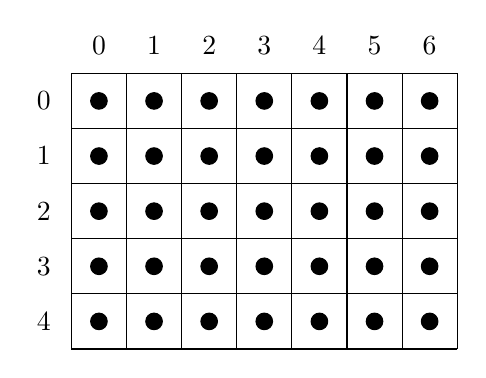
\begin{tikzpicture}[scale=\scale]
 % x coordinates
 \pgfmathparse{\xwidth-1}
 \foreach \x in {0,...,\pgfmathresult}
  \node at (\x+.5,\ywidth+.5) {\x};
 % y coordinates
 \pgfmathparse{\ywidth-1}
 \foreach \y in {0,...,\pgfmathresult}
  \node at (-.5,\ywidth-\y-.5) {\y};
 % Vertical lines
 \foreach \x in {0,...,\xwidth}
  \draw (\x,0) -- (\x,\ywidth);
 % Horizontal lines
 \foreach \y in {0,...,\ywidth}
  \draw (0,\y) -- (\xwidth,\y);
 % "Values"
 \foreach \x in {1,...,\xwidth}
  \foreach \y in {1,...,\ywidth}
   \draw[fill=black] (\x-.5,\y-.5) circle (.15);
\end{tikzpicture}
} \qquad
 \subfloat[Vertex-centered]{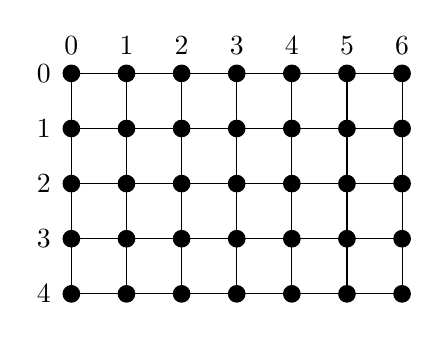
\begin{tikzpicture}[scale=\scale]
 % x coordinates
 \pgfmathparse{\xwidth-1}
 \foreach \x in {0,...,\pgfmathresult}
  \node at (\x,\ywidth-.5) {\x};
 % Vertical lines
 \foreach \x in {0,...,\pgfmathresult}
  \draw (\x,0) -- (\x,\ywidth-1);
 % y coordinates
 \pgfmathparse{\ywidth-1}
 \foreach \y in {0,...,\pgfmathresult}
  \node at (-.5,\pgfmathresult-\y) {\y};
 % Horizontal lines
 \foreach \y in {0,...,\pgfmathresult}
  \draw (0,\y) -- (\xwidth-1,\y);
 % "Values"
 \foreach \x in {1,...,\xwidth}
  \foreach \y in {1,...,\ywidth}
   \draw[fill=black] (\x-1,\y-1) circle (.15);
\end{tikzpicture}
}
 \caption{Cell-centered and vertex-centered grids}
 \label{fig:cell-centered vertex-centered}
\end{figure}


\subsection{NetCDF files}
\label{sec:netcdf files}

All NetCDF files opened with ASAGI should respect the COARDS conventions\footnote{\url{http://ferret.wrc.noaa.gov/noaa_coop/coop_cdf_profile.html}}. However, ASAGI has some further limitations:
\begin{itemize}
 \item The attributes \texttt{scale\_factor} and \texttt{add\_offset} are ignored. Besides conversion between data types, ASAGI does not modify the values.
 \item Since ASAGI does not change the NetCDF file, all values have to be present in the file. Attributes, like \texttt{\_FillValue} and \texttt{missing\_value}, are not supported.
 \item ASAGI is not aware of any units. It is up to the user of the library to interpret the values correctly.
 \item Variables with more than three dimensions are not supported.
\end{itemize}

It is possible to open a NetCDF file by different grids or levels at the same time. This allows you, for example, to store all levels of one grid in a single NetCDF file. In this case the levels must be distinguished by the variable names.

\subsection{Multi-thread support}

When compiled with \texttt{THREADSAFTY=ON} (see section \ref{sec:compilation}) all functions are thread-safe. However, there are some restrictions due to MPI implementations. To receive values from a grid with different threads MPI must support at least \texttt{MPI\_THREAD\_SERIALIZED}. If you want to \texttt{open} or \texttt{close} several grids at the same time, support for \texttt{MPI\_THREAD\_MULTIPLE} is required.

\def\interfacefiles{group__c__interface,group__cxx__interface,group__f__interface}

\sloppy

\foreach \interfacefile in \interfacefiles
{
 \InputIfFileExists{interfacedoc/\interfacefile}{}{}
}

\fussy
